\chapter{Modelos baseados em \textit{Bag of Words}} \label{bow_implementation}

Para a representação \textit{bag of words}, foram utilizados algoritmos classificadores tradicionais conforme descrito em \cite{InformationRetrievalBook}. Eles atuam como uma referência de \textit{benchmarking} para os modelos mais modernos que serão discutidos na seção \ref{We_implementation}.

Como etapas de preparação da estrutura de dados a partir da representação \textit{bag of words}, foram utilizadas as seguintes técnicas de processamento de linguagem natural do pacote NLTK (\textit{Natural Language Toolkit}), que possui suporte para a linguagem português brasileiro: a separação da frase em palavras, deixando-as com letra minúscula; a remoção de \textit{stopwords} (palavras de parada) desse conjunto de palavras, apresentadas no apêndice \ref{stopwords}; e a lematização das palavras utilizando \textit{RSLPStemmer} (Removedor de Sufixos da Língua Portuguesa) (\cite{RSLPStemmer}). Após a aplicação dessas técnicas, é utilizado TF-IDF por meio da implementação \textit{TfidfTransformer} da biblioteca \textit{scikit-learn}.

\section{\textit{Naive Bayes}}

Conforme descrito na seção \ref{theoretical_NB}, o classificador NB foi um dos utilizados para a representação textual \textit{bag of words}. A versão utilizada nessa implementação foi a variante multinomial que, como o próprio sugere, assume uma distribuição multinomial na inferência de probabilidade. Utilizou-se a implementação da biblioteca do \textit{scikit-sklearn}, obtendo-se resultados sumarizados pela figura \ref{fig:confusion_matrix_NB} e pela tabela \ref{tab:NB}.

\begin{table}[ht]
\centering
\caption{Métricas do modelo \textit{naive bayes}}
\vspace{0.5cm}
\begin{tabular}{c|c|c}
 
Métrica & Conj. de Treinamento & Conj. de Teste \\
\hline
Acurácia & 0.79287 & 0.78655 \\
F1-Score & 0.77180 & 0.76427 \\
Precisão & 0.80543 & 0.79806 \\
AUC ROC  & 0.97163 & 0.96980
\end{tabular}
\label{tab:NB}
\end{table}

\begin{figure}[!ht]
	\centering
	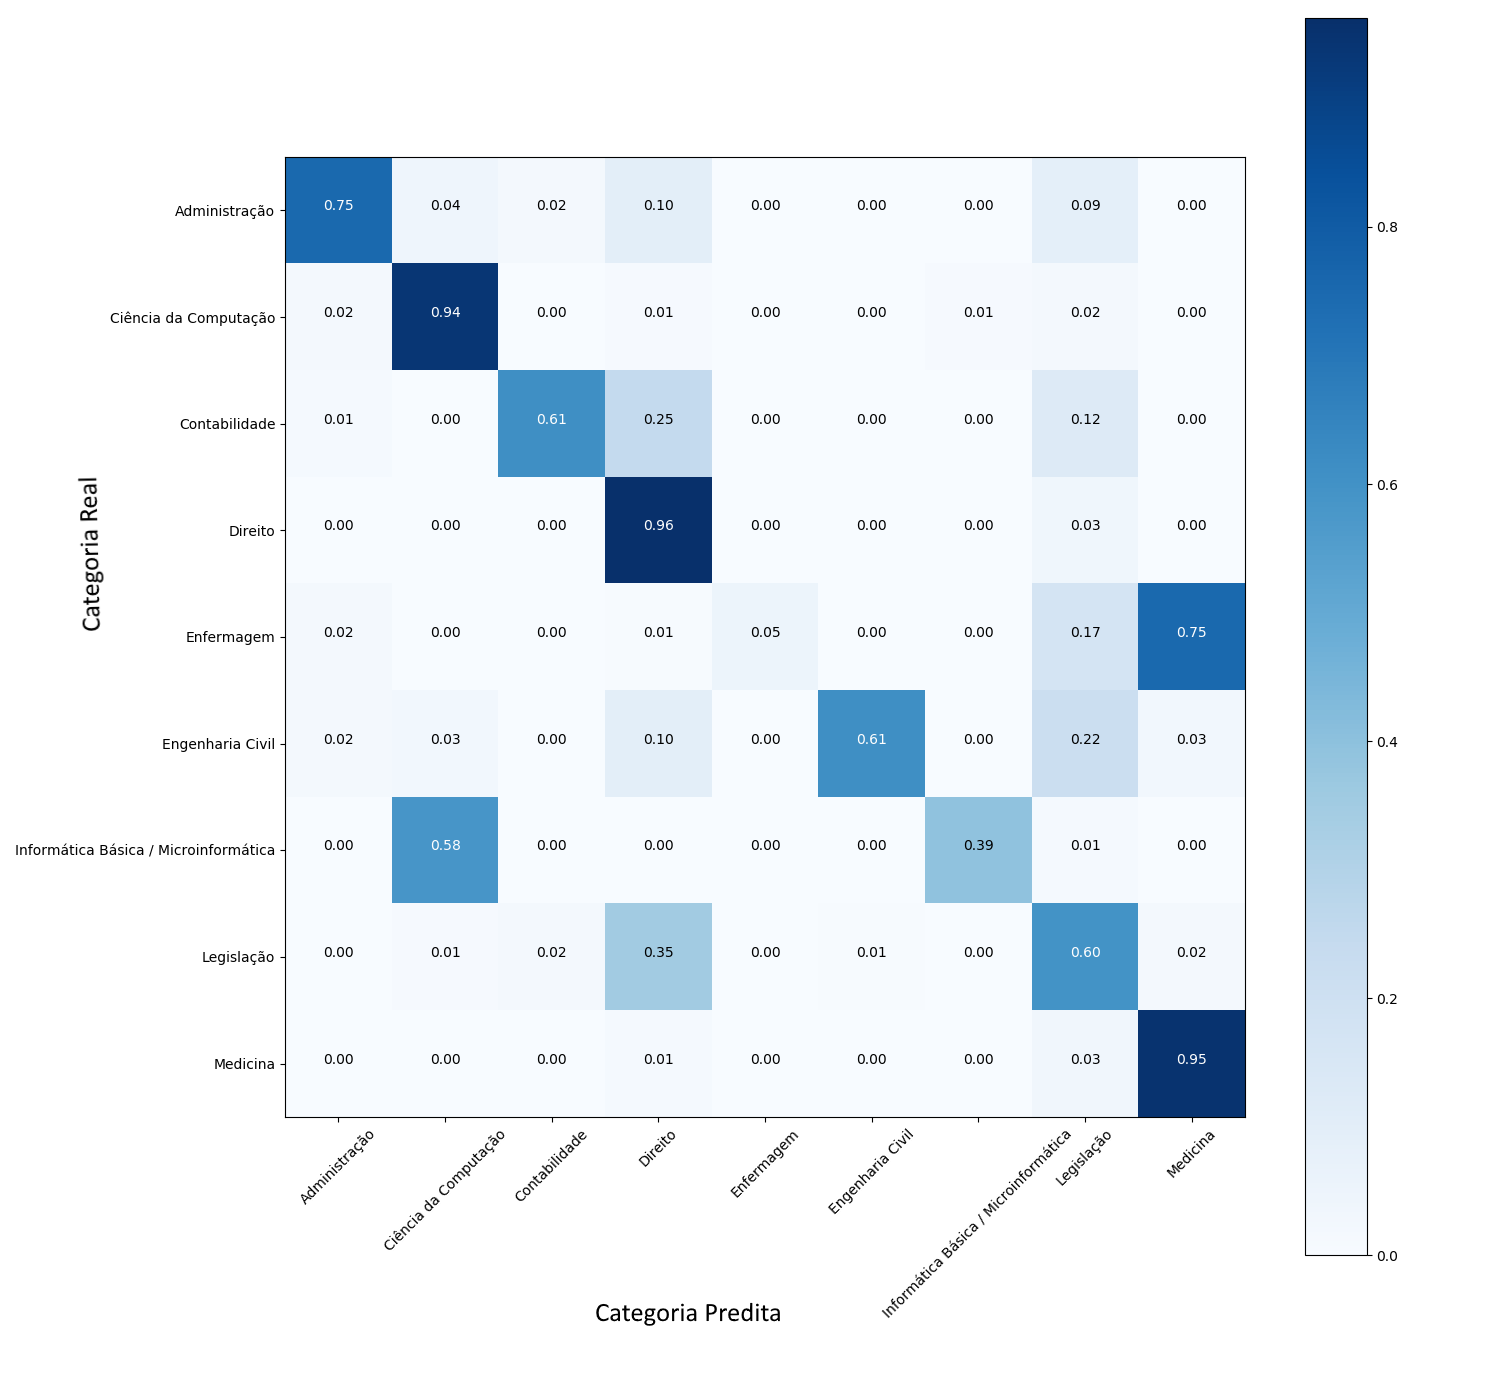
\includegraphics[width=1.1\textwidth]{figures/NB_-_Confusion_matrix_normalized_-_test.png}
	\caption{Matriz de confusão do conjunto de testes normalizada para o classificador Naive Bayes}
	\label{fig:confusion_matrix_NB}
\end{figure}

\section{\textit{Support Vector Machines}}

O segundo classificador para o modelo \textit{bag of words} foi o classificador SVM, descrito na seção \ref{theoretical_SVM}. A implementação escolhida para esse classificador foi também a da biblioteca \textit{sklearn} a partir do método \textit{SGDClassifier}, resultando na matriz de confusão da figura \ref{fig:confusion_matrix_SVM} em que as métricas são detalhadas pela tabela \ref{tab:SVM}.

\begin{table}[ht]
\centering
\caption{Métricas do modelo \textit{SVM}}
\vspace{0.5cm}
\begin{tabular}{c|c|c}
 
Métrica & Conj. de Treinamento & Conj. de Teste \\
\hline
Acurácia & 0.77368 & 0.77295 \\
F1-Score & 0.74712 & 0.74489 \\
Precisão & 0.78709 & 0.78676
\end{tabular}
\label{tab:SVM}
\end{table}

\begin{figure}[!ht]
	\centering
	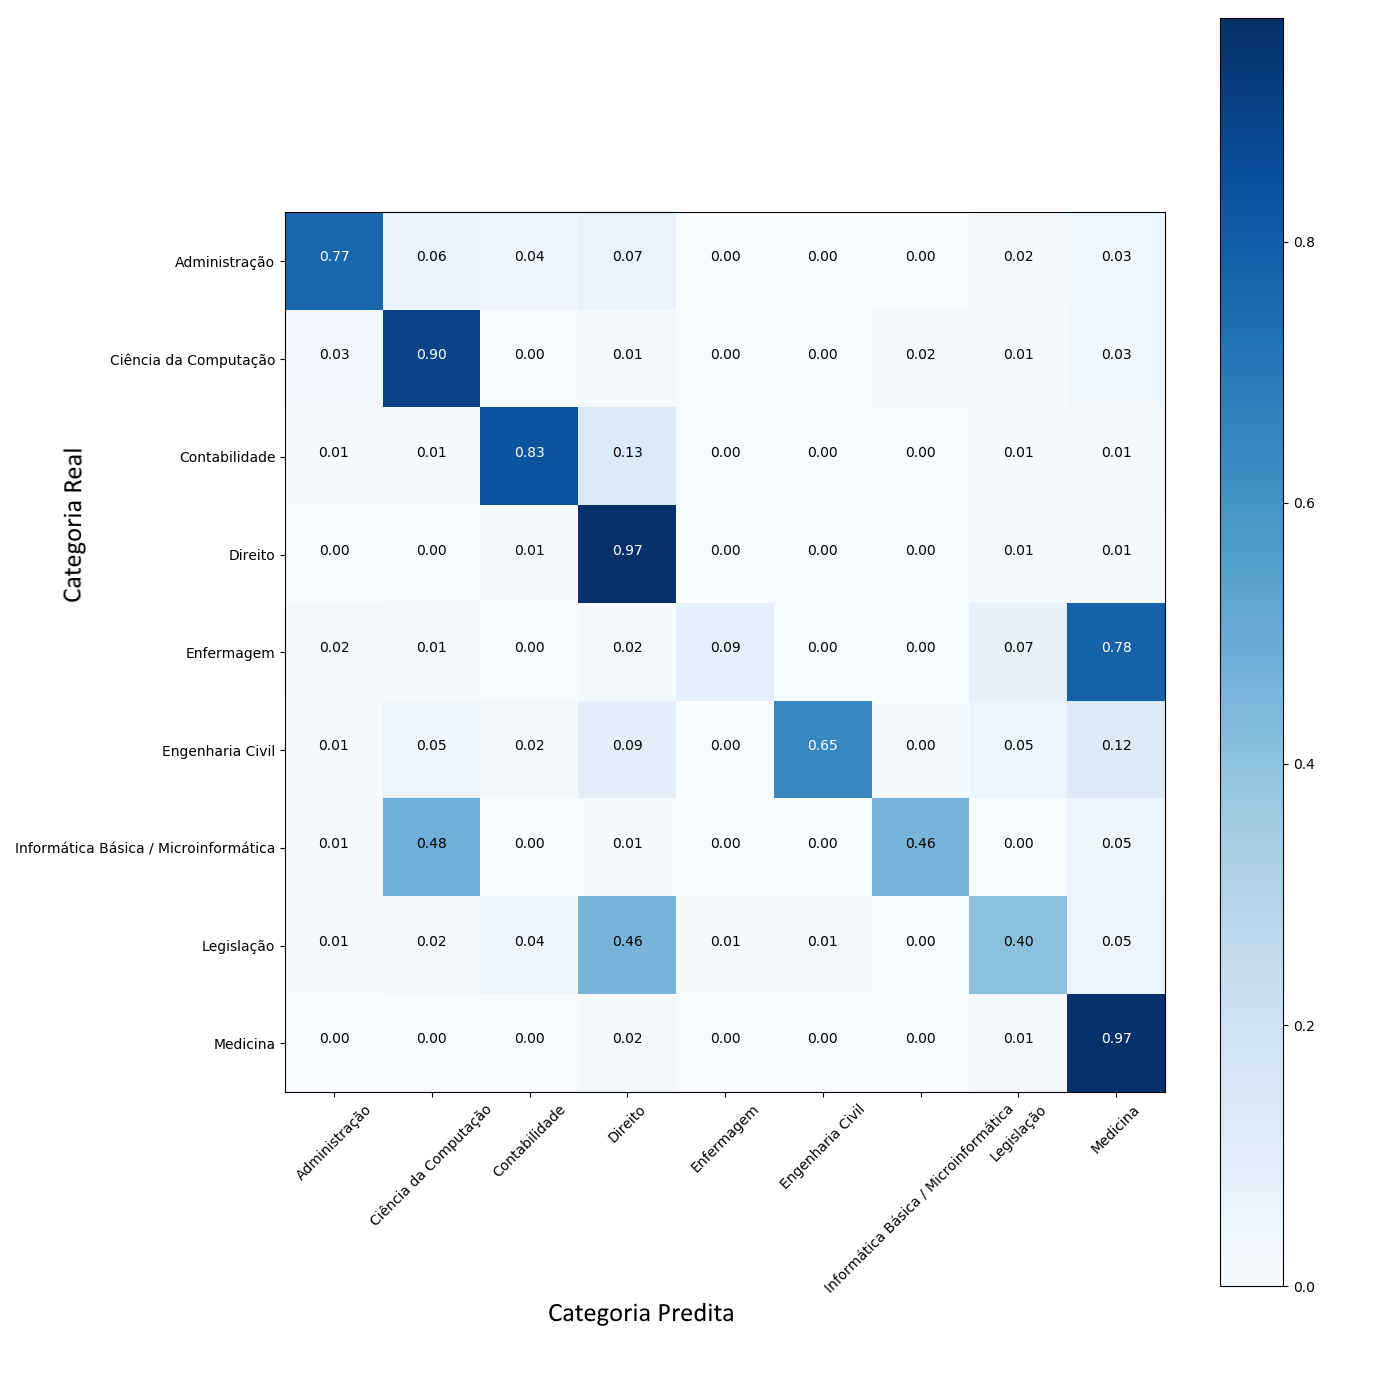
\includegraphics[width=1.1\textwidth]{figures/SVM_Confusion_matrix_normalized.png}
	\caption{Matriz de confusão do conjunto de testes normalizada para o classificador SVM}
	\label{fig:confusion_matrix_SVM}
\end{figure}